\chapter{Sand extraction}
Sand extraction in the Lower Paraná Delta occurs both on land and in the river. Therefore, dredging activities as well as dry sand mining are considered. The purpose of this chapter is to make an assessment of extraction quantities and evaluate the relative importance of the both types of sand extraction. 

\section{Dredging activities}
This section describes the relevance of dredging to the sediment balance of the designated area, by an estimation of the dredging quantities in the river. This will be done by analysing AIS data and extraction permits that were submitted to INA.

\subsection{Vessel positioning information (AIS)}
Using MarineTraffic it was found that two dredgers are operating on the Paraná Guazú between Ibicuy and Brazo Largo: the Comercio Segundo and the E.M. Arroyo N1. The Comercio Segundo has a length of 30 m, a width of 7 m, a draft of 1.3 m, and an approximate cargo hold of 195 m\textsuperscript{3}. The E.M. Arroyo N1 has a length of 39 m, a width of 8 m, a draught of 2.8 m and an approximate cargo hold of 476 \,m\textsuperscript{3}. Using a sand to water ratio of 3:1 for the dredged slurry, the amount of sand dredged is 150 \,m\textsuperscript{3} and 360 \,m\textsuperscript{3} respectively per cargo. The tracks of the two vessels obtained from MarineTraffic are shown in Figure \ref{fig:track_cs} and Figure \ref{fig:track_em}.

\begin{figure}[H]
    \centering
    \begin{minipage}{0.48\textwidth}
        \centering
        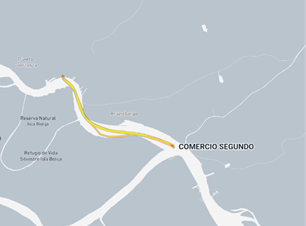
\includegraphics[width=\linewidth]{figures/ch5/Track_CS.png}
        \caption{Track of the \textit{Comercio Segundo}}
        \label{fig:track_cs}
    \end{minipage}\hfill
    \begin{minipage}{0.48\textwidth}
        \centering
        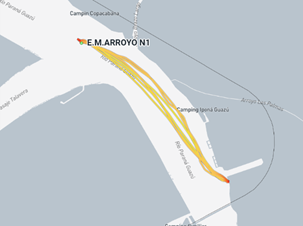
\includegraphics[width=\linewidth]{figures/ch5/Track_EM.png}
        \caption{Track of the \textit{E.M. Arroyo N1}}
        \label{fig:track_em}
    \end{minipage}
\end{figure}

The AIS data for these two vessels is obtained from MyShipTracking, which is used to determine the location of the dredging and the average number of trips. The dredging location of the two vessels is shown in Figure \ref{fig:dredging_coordinates}. It can be seen that both dredgers operate in the same area. This can be explained by the bathymetry shown in Figure \ref{fig:bathymetry}, which shows a reduced depth near the junction of the two navigable channels. At this location the flow velocity is lower, causing sediment to settle and thus creating a sandbar. From the AIS data it was concluded that both dredgers make three trips per day.

\begin{figure}[H]
    \centering
    \begin{minipage}{0.48\textwidth}
        \centering
        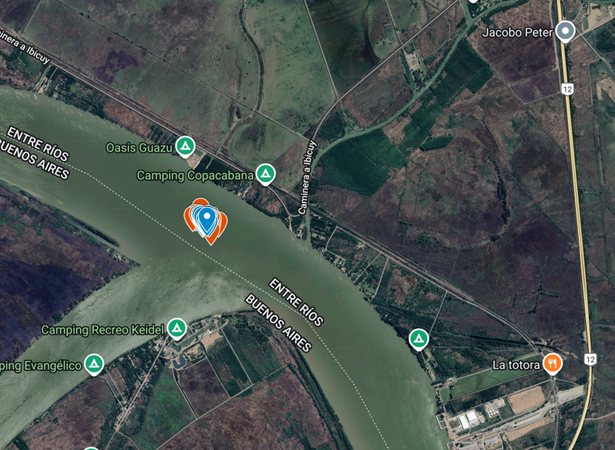
\includegraphics[width=\linewidth]{figures/ch5/Dredging_coordinates.png}
        \caption{Dredging location}
        \label{fig:dredging_coordinates}
    \end{minipage}\hfill
    \begin{minipage}{0.48\textwidth}
        \centering
        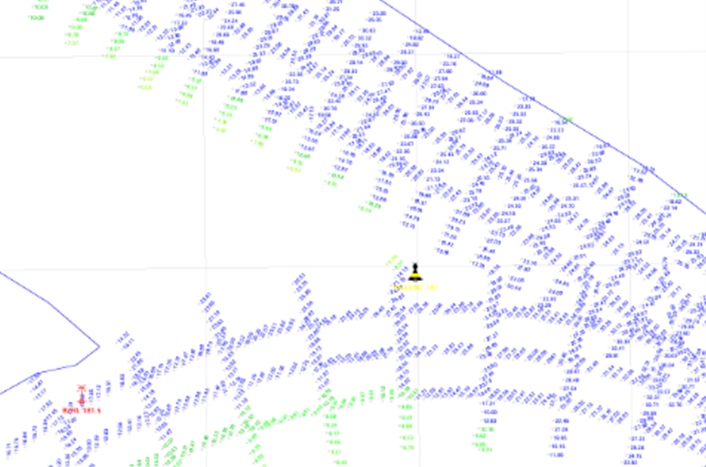
\includegraphics[width=\linewidth]{figures/ch5/Bathymetry.png}
        \caption{Bathymetry}
        \label{fig:bathymetry}
    \end{minipage}
\end{figure}

In the Rio Talabera, a side branch connecting to the Paraná Guazú, a third dredger is extracting sand. The Altair is a dredging vessel with a length of 66 m, a width of 11 m, a draught of 1.5 m and an approximate cargo hold of 750 \,m\textsuperscript{3}. Using the same sand to water ratio of 3:1 this gives 560 \,m\textsuperscript{3} of sand per cargo. Using MarineTraffic it was found that the Altair makes 3 trips per day on average. Figure \ref{fig:Altair_track} shows the its track and the location at which it halts to extract sand. For all three vessels that were identified in the study area, the estimated volume of sand extracted per month is displayed in Table \ref{tab:sand_volume}.

\begin{figure}[H]
    \centering
    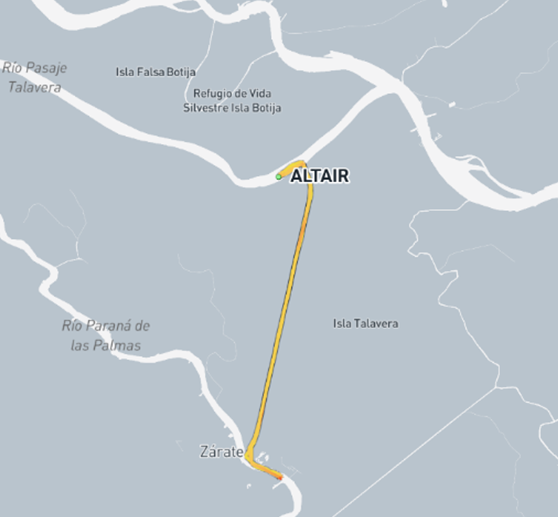
\includegraphics[width=0.5\linewidth]{figures/ch5/Track_Altair.png}
    \caption{Track of the Altair}
    \label{fig:Altair_track}
\end{figure}


\begin{table}[h!]
\centering
\begin{tabular}{lrrrr}
\hline
\textbf{Vessel} & \textbf{Cargo hold [\,m\textsuperscript{3}]} & \textbf{Sand volume [\,m\textsuperscript{3}]} & \textbf{Trips per day} & \textbf{Volume per month [\,m\textsuperscript{3}]} \\
\hline
Comercio Segundo & 195 & 150 & 3 & 9000 \\
E.M. Arroyo N1 & 476 & 360 & 3 & 21600 \\
Altair & 750 & 560 & 3 & 33600 \\
\hline
\end{tabular}
\caption{Sand transport details per vessel.}
\label{tab:sand_volume}
\end{table}

\subsection{Extraction permits}
A total of 33 permits were collected for the Paraná Guazú and 43 for the Ibicuy. On the Paraná Guazú, four permits were issued for channel maintenance, while the remainder concerned sand extraction. For the Ibicuy, all permits were related to extraction activities. The analysis shows that the requested volumes in the Ibicuy are considerably larger than those in the Paraná Guazú, even though the section of the Ibicuy considered here is much shorter in length: Paraná Guazú stretches from km 124.0 to km 232.0, Ibicuy from km 232.0 to approximately km 249.0 for the area of interest (\cite{AGPComenzoBatimetria2023}).

It is important to note that the end dates of contracts are unknown. While the requests specify monthly dredging quantities, they do not indicate the duration of the works. As a result, a detailed quantitative assessment cannot be made. For the present analysis, all requests with fixed monthly volumes are assumed to extend over 12 months. The second assumption is to record a single value for the requested volume, when information about monthly or yearly occurrence is lacking. This allows for a comparison between the two river sections of yearly extraction volumes, as shown in Figure \ref{fig:yearly dredging volumes}. As mentioned, sand extraction activities on the Ibicuy are large compared to Paraná Guazú, with a maximum recorded yearly volume of almost $4 \cdot 10^6 ~m^3$.  

\begin{figure}[H]
    \centering
    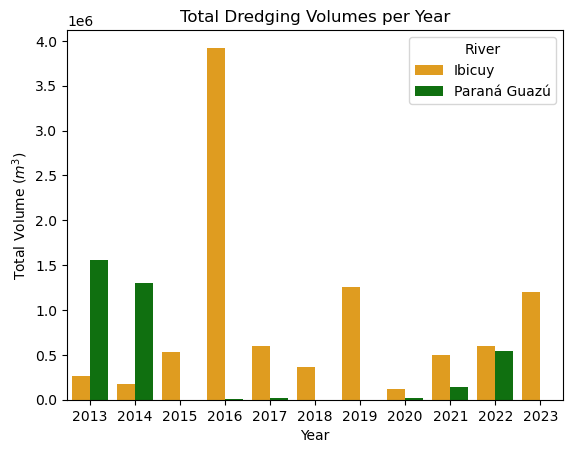
\includegraphics[width=0.50\linewidth]{figures/ch2/Dredging volumes permits.png}
    \caption{Yearly dredging volumes}
    \label{fig:yearly dredging volumes}
\end{figure}

\subsection{Estimated sand extraction}
This section draws a conclusion on the sand extraction volumes, such that an estimate is found to apply in the sediment balance. Based on the AIS data, permits and stakeholder interviews, the following uncertainties were considered in determining a representative value:

\begin{itemize}
    \item Not every vessel in the area is equipped with an AIS transponder, meaning that possibly not all active vessels were identified. However, the number of vessels as found by analysis of the AIS data was in agreement with the number of vessels observed during the fieldwork.
    \item No historical AIS data was available, such that the data was registered for only a short period of time.
    \item The extraction permits do not mention the duration of the contract.
    \item Whereas permits imply that most of the activity occurs on the Ibicuy, AIS data and fieldwork observations indicate that the activity on the Paraná Guazú is higher. 
    \item Stakeholders stress that activity on the Ibicuy has ceased, as described in Section \ref{subsec:dredging activities interviews}.
\end{itemize}

However, a rough estimate can be found by calculating the mean annual volume for the total system of interest (i.e., Ibicuy and Paraná Guazú) based on the extraction permits. To make a comparison with the monthly values in Table \ref{tab:sand_volume}, this yearly value is reduced to a monthly value by dividing by 12 months. The former approach yields the following value for dredged sand volumes:

\begin{equation}
    V_{sand,yearly} = 1193923 ~m^3
\end{equation}
\begin{equation}
\label{eq:monthly extraction}
    V_{sand,monthly} = \frac{V_{sand,yearly}}{12} \approx 100000 ~m^3
\end{equation}

Summation of the monthly volumes in Table \ref{tab:sand_volume} gives a monthly total of $64200 ~m^3$. Considering that not all vessels have AIS transponders, a conservative estimate of $V_{sand,monthly}$ will be used as calculated in Equation \ref{eq:monthly extraction}.

\section{Dry sand mining}
As mentioned in chapter \ref{chapter:stakeholders}, many stakeholders stressed the relevance of dry sand mining related to fracking for the lower delta region. In this section, context to these claims is given. The history and development of fracking in Argentina is discussed, followed by the related sand mining. Then, geological properties of the area of interest are looked into as well as the characteristics of dry sand used in fracking. Finally, the effects of dry sand mining are discussed and recommendations plus mitigation strategies are given.

\subsection{Fracking in Argentina}
\label{sec: fracking in argentina}
For much of its history, Argentina was regarded as a modest oil producer, struggling to meet its own energy demands. This perception shifted with the 2010 discovery of the Vaca Muerta shale formation, located in the Neuquén basin in Patagonia. The Argentine energy company YPF then identified approximately 150 million barrels of recoverable oil in the field, which was regarded as a new source of hope for economic stability by some, among whom was the president \autocite{kraussArgentinaHopesBig2011}.

The discovery was followed by significant foreign investment. More exploration was done and now it is clear that Argentina possesses the world’s fourth-largest shale oil and second-largest shale gas reserves \autocite{internationaltradeadministrationArgentinaCountryCommercial2025}. Today, around thirty companies hold licenses to exploit various areas of the Vaca Muerta basin. The biggest operator is a consortium of YPF, a majority state-owned Argentine energy company, and Chevron, an American energy company. Other players are Tecpetrol, Total, Dow Petrochemical, Petronas, Shell, Gazprom, and ExxonMobil \autocite{fogliaSedArena2023}.

The Nuequén basin is located in the provinces of Neuquén, Mendoza, and Río Negro in the South of Argentina and has been an important basin for oil and gas since more than a century. Production started in 1918 and in 2004, 45\% of Argentinian oil production and 61\% of its gas production came from this area \autocite{u.s.energyinformationadministrationTechnicallyRecoverableShale2013}. This was done through conventional methods, but after the discovery of the Vaca Muerta shale basin, fracking has become increasingly important for the region and the country. The Vaca Muerta shale consists of finely-stratified black to dark grey shale and lithographic lime-mudstone and is 60 to 520 m thick. Estimates are that the formation contains 16 billion barrels of technically recoverable oil and 8722 billion cubic metres of technically recoverable gas \autocite{u.s.energyinformationadministrationTechnicallyRecoverableShale2013}. Since Vaca Muerta is a shale reservoir, all oil and gas from this deposit is extracted by fracking.

As can be seen in figure \ref{fig:oilgasprod}, oil production in Argentina has been steadily increasing since 2020, driven by increased production of the Vaca Muerta formations. After the exploration in 2010, oil from Vaca Muerto as a share of total Argentinian oil production has increased from virtually 0\% to 55\% today. Further, Vaca Muerta now accounts for 47\% of gas supply \autocite{internationaltradeadministrationArgentinaCountryCommercial2025}.

\begin{figure}[H]
    \centering
    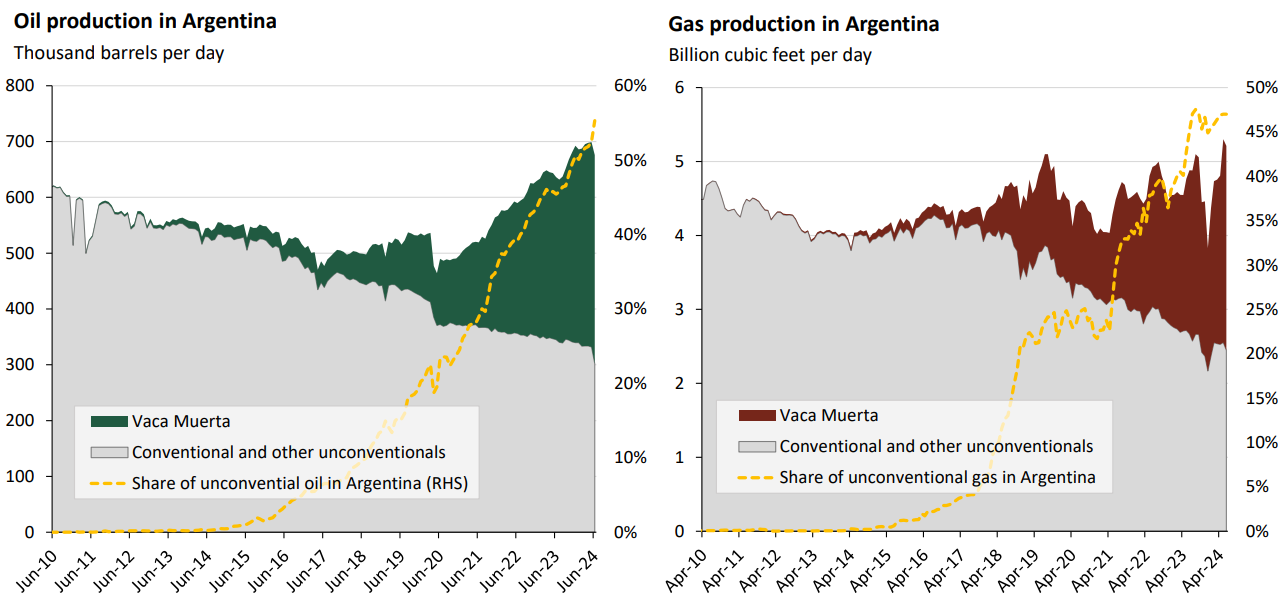
\includegraphics[width=1\linewidth]{figures/ch9/oilgasproduction.png}
    \caption{Oil and gas production in Argentina \autocite{internationaltradeadministrationArgentinaCountryCommercial2025}}
    \label{fig:oilgasprod}
\end{figure}

The numbers in figure \ref{fig:oilgasprod} help explain why fracking in the Neuquén basin is viewed by some as critical to the development of Argentina's economy. In fact, the Government of Argentina still views the oil and gas sector as a crucial part of its economy, by driving exports as well as generating foreign currency and investment. It also becomes clear that, considering the volumes present in the reserves, even more gas and oil could still be extracted.

\subsection{Theoretical background: fracking}
In the 1970's, geologists became increasingly aware that large volumes of gas existed in low-permeability sandstones. However, conventional methods did not allow for economic extraction of gas from these `tight reservoirs' \autocite{lawGasTightReservoirs1992}. Hydraulic fracturing, or fracking, a method first tested in 1947 and applied on a large scale for the first time in the 1970's, is used to extract oil and natural gas from these low-permeability rock formations, such as shale \autocite{denchakFracking1012019}.

The technique begins by drilling a long vertical well. As soon as the desired rock formation is reached, drilling gradually turns horizontal and steel pipes called `casings' are inserted into the well. Small holes are perforated in the casing and then fracking fluid is pumped in at a pressure high enough to create new fractures or open existing ones in the surrounding rock. This allows previously unavailable oil or gas to flow to the surface \autocite{denchakFracking1012019}.

The fracking fluid contains as much as 97 percent water, but also always contains proppants. These are small, solid particles that keep the fractures in the rock formation open after the pressure from injection is removed. Sand, or more specifically silica sand, is the most widely-used proppant in the fracking industry \autocite{denchakFracking1012019}. Sand is thus an essential substance to keep the drilled pores open and to allow for the fossil fuels to flow out.

\subsection{Sand mining practices}
The sand used in fracking is mined or imported. In figure \ref{fig:sanddiagram}, the mined silica sand masses as well as the imported masses are given for Argentina. This includes sand used for fracking but also other purposes.

\begin{figure}[H]
    \centering
    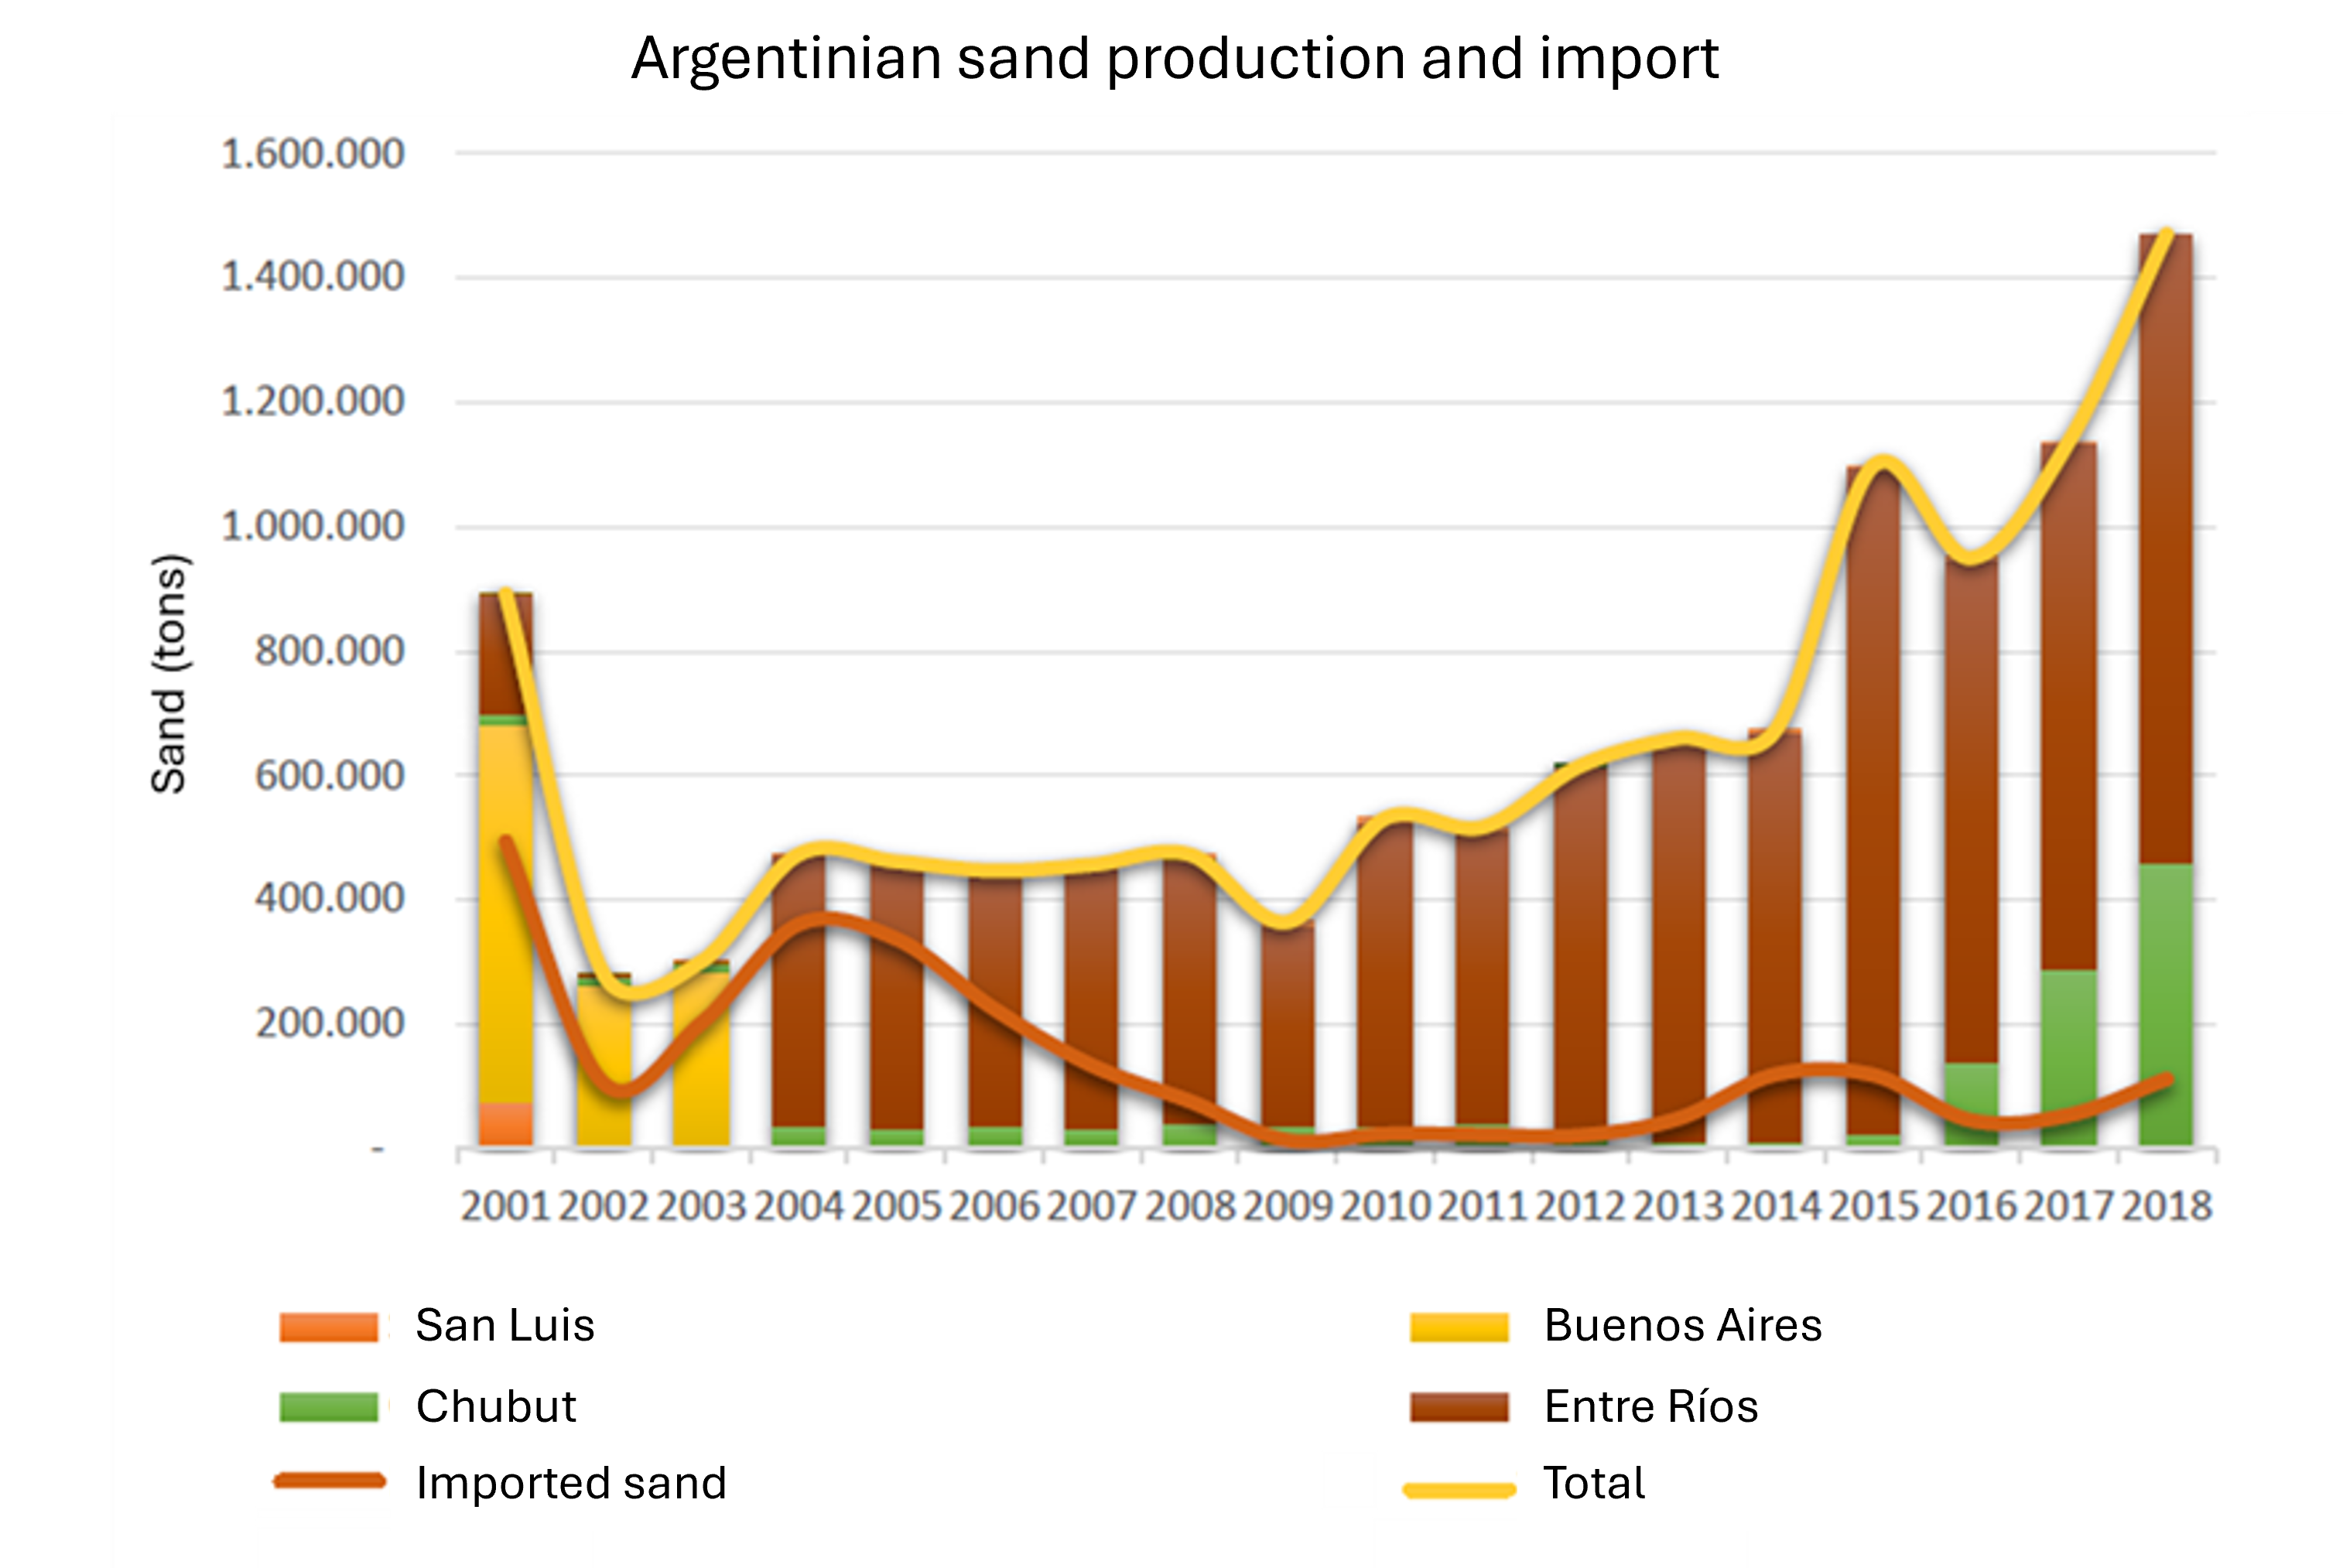
\includegraphics[width=1\linewidth]{figures/ch9/Sandgraphquantities.png}
    \caption{Quantities of sand mined in Argentine provinces, adapted from \cite{secretariadepoliticamineraArenasParaFracking2019}}
    \label{fig:sanddiagram}
\end{figure}

In 2018, approximately 1.5 million tons of sand was produced and imported in Argentina, with more than 90\% of used sand from national origin. Of the nationally mined sand, 69\% had its origin in Entre Ríos \autocite{secretariadepoliticamineraArenasParaFracking2019}. Specific numbers for the period after are unavailable, but in 2020, the amount of sand needed in Argentina was 3.5 million tons \autocite{novasImpactoAmbientalOculto2022}. This indicates that the upgoing trend has since persisted.

Historically, silica sand was used as a raw material for the glass industry but since the introduction of fracking, sand miners have found a new purpose for their product. The exact volumes of sand used for fracking versus the volumes used for other purposes are unknown. However, as can be seen in figure \ref{fig:sanddiagram}, the upgoing trend in sand production can be observed only for the past years, after the discovery of Vaca Muerta. It seems therefore clear that fracking practices are the driving force behind the increasing demand of sand. This is also the conclusion that other reports reach \autocite{secretariadepoliticamineraArenasParaFracking2019} \autocite{fogliaSedArena2023}.

\subsection{Sand mining in the lower delta}
During the fieldwork and by using satellite data, the locations of sand mines in the lower delta were identified. A total of 11 locations were found, 10 of which fall within the department of Islas del Ibicuy. In figure \ref{fig:sandminemap} the locations are shown and in figure \ref{fig:sandminessatellite}, the aerial view is given for three sand mines in the department of Ibicuy.

\begin{figure}[H]
    \centering
    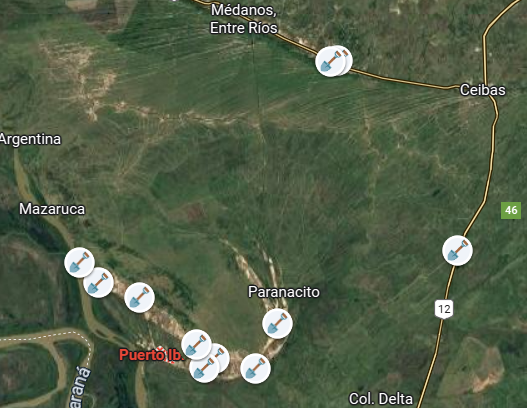
\includegraphics[width=0.6\linewidth]{figures/ch9/SandMap.png}
    \caption{The identified locations of sand mines}
    \label{fig:sandminemap}
\end{figure}

\begin{figure}[H]
    \centering
    \includegraphics[width=1\linewidth]{figures/ch9/Sandminessatellite.png}
    \caption{Examples of sand mines in the department of Ibicuy}
    \label{fig:sandminessatellite}
\end{figure}

Of all departments where sand mining takes place, the most intense activities are carried out in Ibicuy. Previous reports estimate that 1.250.000 tons of sand were mined in Ibicuy alone in 2022 \autocite{fogliaSedArena2023}. This number is comparable to the total national sand mining volume in 2018. As mentioned in chapter \ref{chapter:stakeholders}, the mayor of Ibicuy described the following scale during the conducted interview: 350 trucks that transport 9,000 tons of sand each day. With a total of 260 working days per year, this amounts to more than 2.3 million tons of sand transported from Ibicuy in 2025, indicating a further increase as compared to 2022.

In Ibicuy, Cristamine, Aresil S. A., YPF, La Chola II, NRG Argentina, San Marcos Trading, and QSand are among the companies that operate sand mining facilities. Sand mining companies that have been around for longer originally only sold their product to the ceramics and glass industry, but at present many of them exclusively sell to the oil sector. Other companies only opened mines after the demand for fracking sand started to rise. An example is La Chola II, a company with 50 years of experience in river sand mining, that opened a dry sand mine in 2016. This is Silicatos Islas del Ibicuy and from here they transport sand to YPF, the biggest player in Argentina's fracking industry \autocite{fogliaSedArena2023}.

Multiple stakeholders, such as the mayor of Ibicuy and the mine manager, explained that mined sand gets transported by trucks to Añelo, a town in Neuquén that forms the heart of the Vaca Muerta fracking activities. This view is confirmed by various reports \autocite{cauceArenasParaFracking2022} \autocite{secretariadepoliticamineraArenasParaFracking2019}. The route from Ibicuy to Añelo is 1283 km long and takes around 20 hours, including a 2 hour delay for handling of goods \autocite{secretariadepoliticamineraArenasParaFracking2019}. The route is indicated in figure \ref{fig:sandroute}. 

\begin{figure}[H]
    \centering
    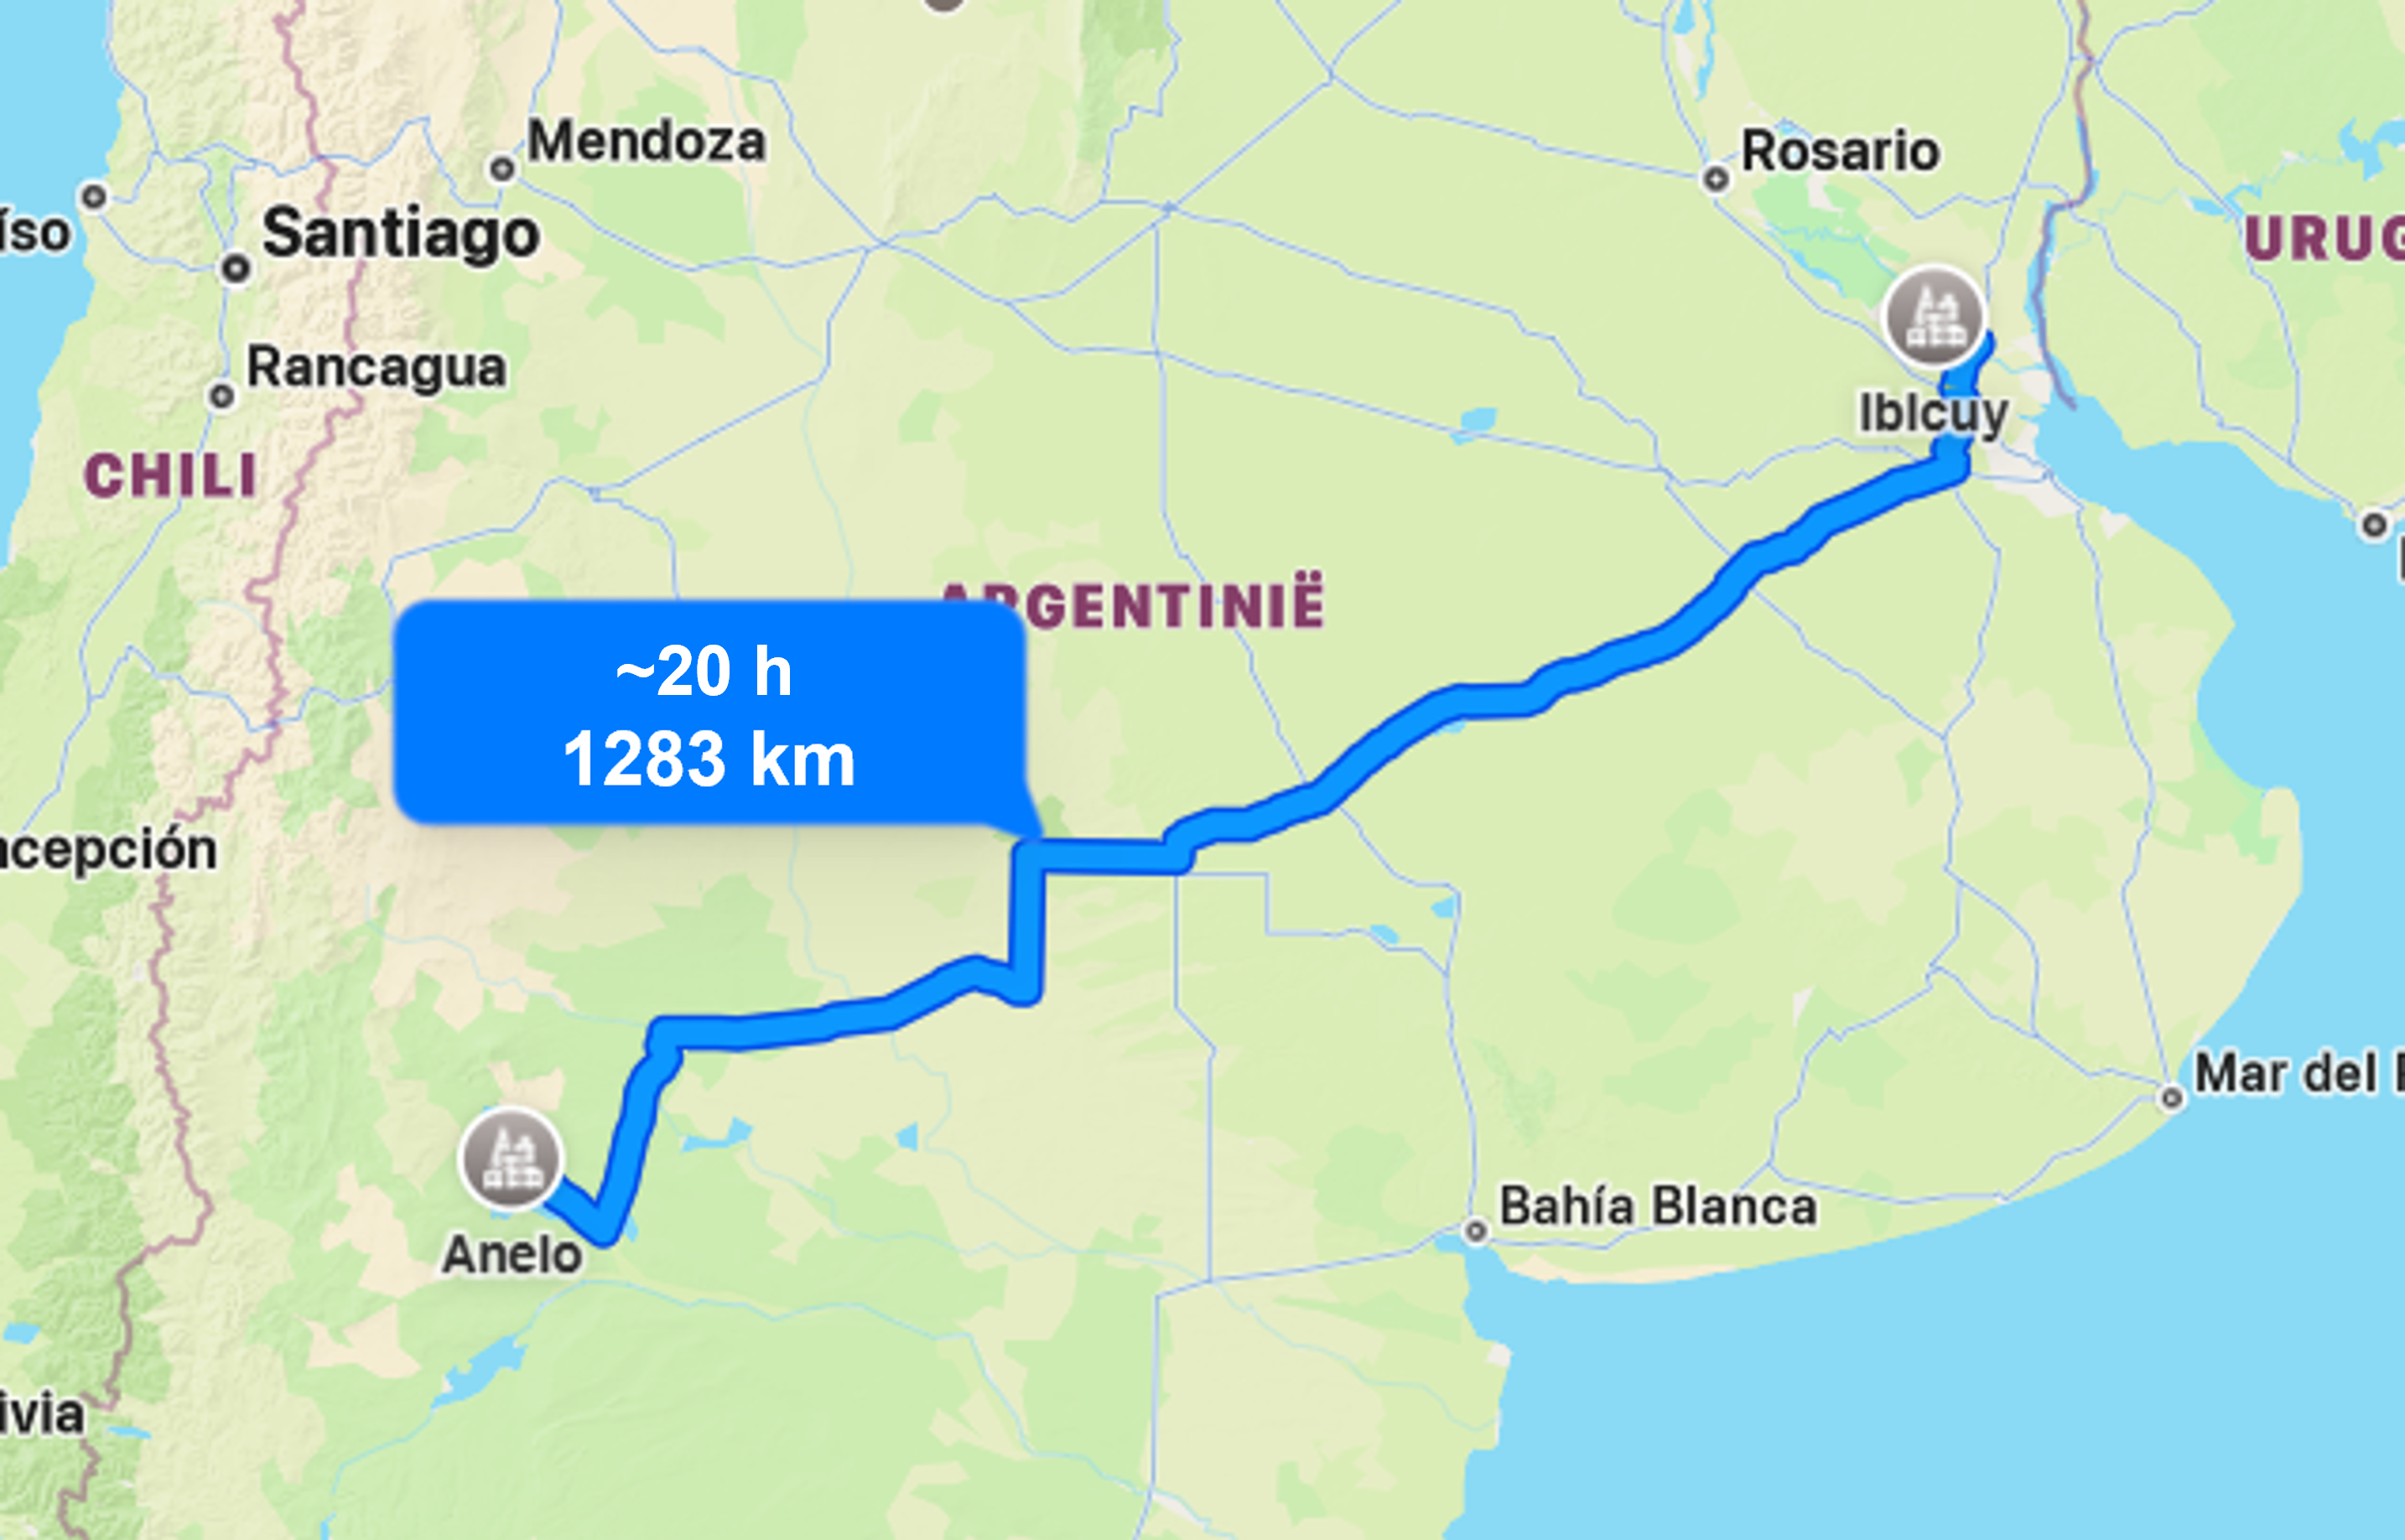
\includegraphics[width=0.6\linewidth]{figures/ch9/Routesand.png}
    \caption{The route from Ibicuy to Añelo}
    \label{fig:sandroute}
\end{figure}

\subsection{Geological conditions} \label{par:geology}
To better understand the dry sand mining activities, the characteristics of the subsoil in the lower delta were researched. This section intends to combine all the available information regarding the subsoil in the investigation area.

\subsubsection{The geology of a delta}
A delta is a landscape formed at the mouth of a river where the water eventually runs into the ocean. At a delta, the water's velocity decreases which gives floating particles in the delta the change to settle. Among these floating particles are gravels, sands and clays, descending in particle size. The particles are formed by erosion of stone. The origin of the particles in the Parana river are the Andes mountains. 
Besides that, deltas are also characterized by high vegetation growth. When this vegetation dies, the organic material will change into peat due to the governing pressures. So, in a delta one expects to find relatively soft soils (sands) and very soft soils (clay and peat).

\subsubsection{Geological cross section}
A study conducted by \citeauthor{joseluiscavallottoEvolucionCambiosAmbientales2005} led to a morphological map of the Paraná delta. In the study, a more detailed geological profile was made for two cross sections, one of which is relevant to the area of interest. The cross section along with the area of interest is shown in figure \ref{fig:crosssectiongeo}.

\begin{figure}[H]
    \centering
    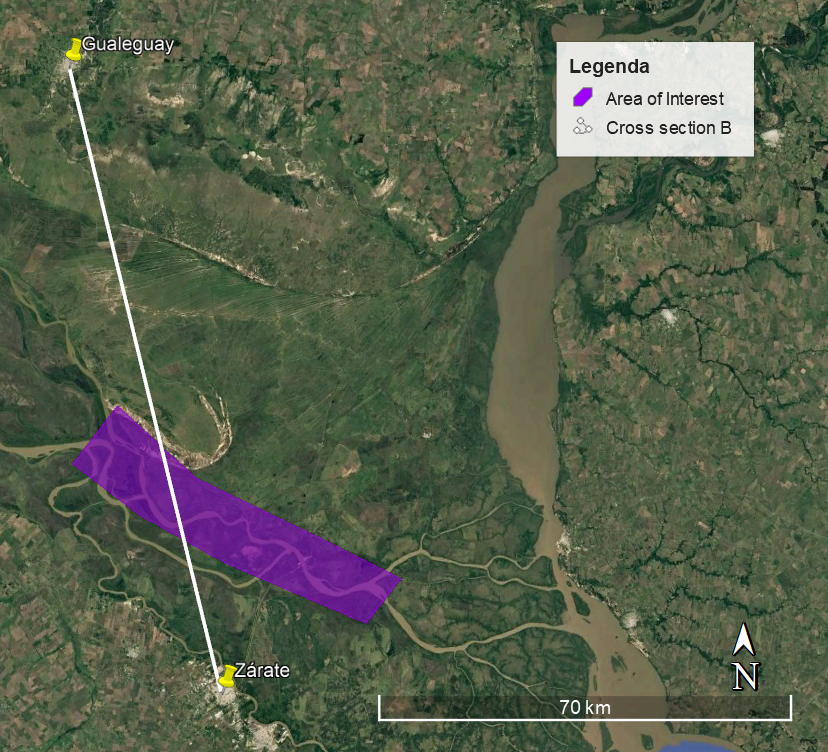
\includegraphics[width=0.75\linewidth]{figures/ch9/CrossSectionB.png}
    \caption{Cross section}
    \label{fig:crosssectiongeo}
\end{figure}

The geological profile of the cross section is shown in figure \ref{fig:geolprofile}. As can be seen in the figure, the taken cross section was around 80 km long. Of this, 15 km falls inside the area of interest, this zone is marked with purple.

\begin{figure}[H]
    \centering
    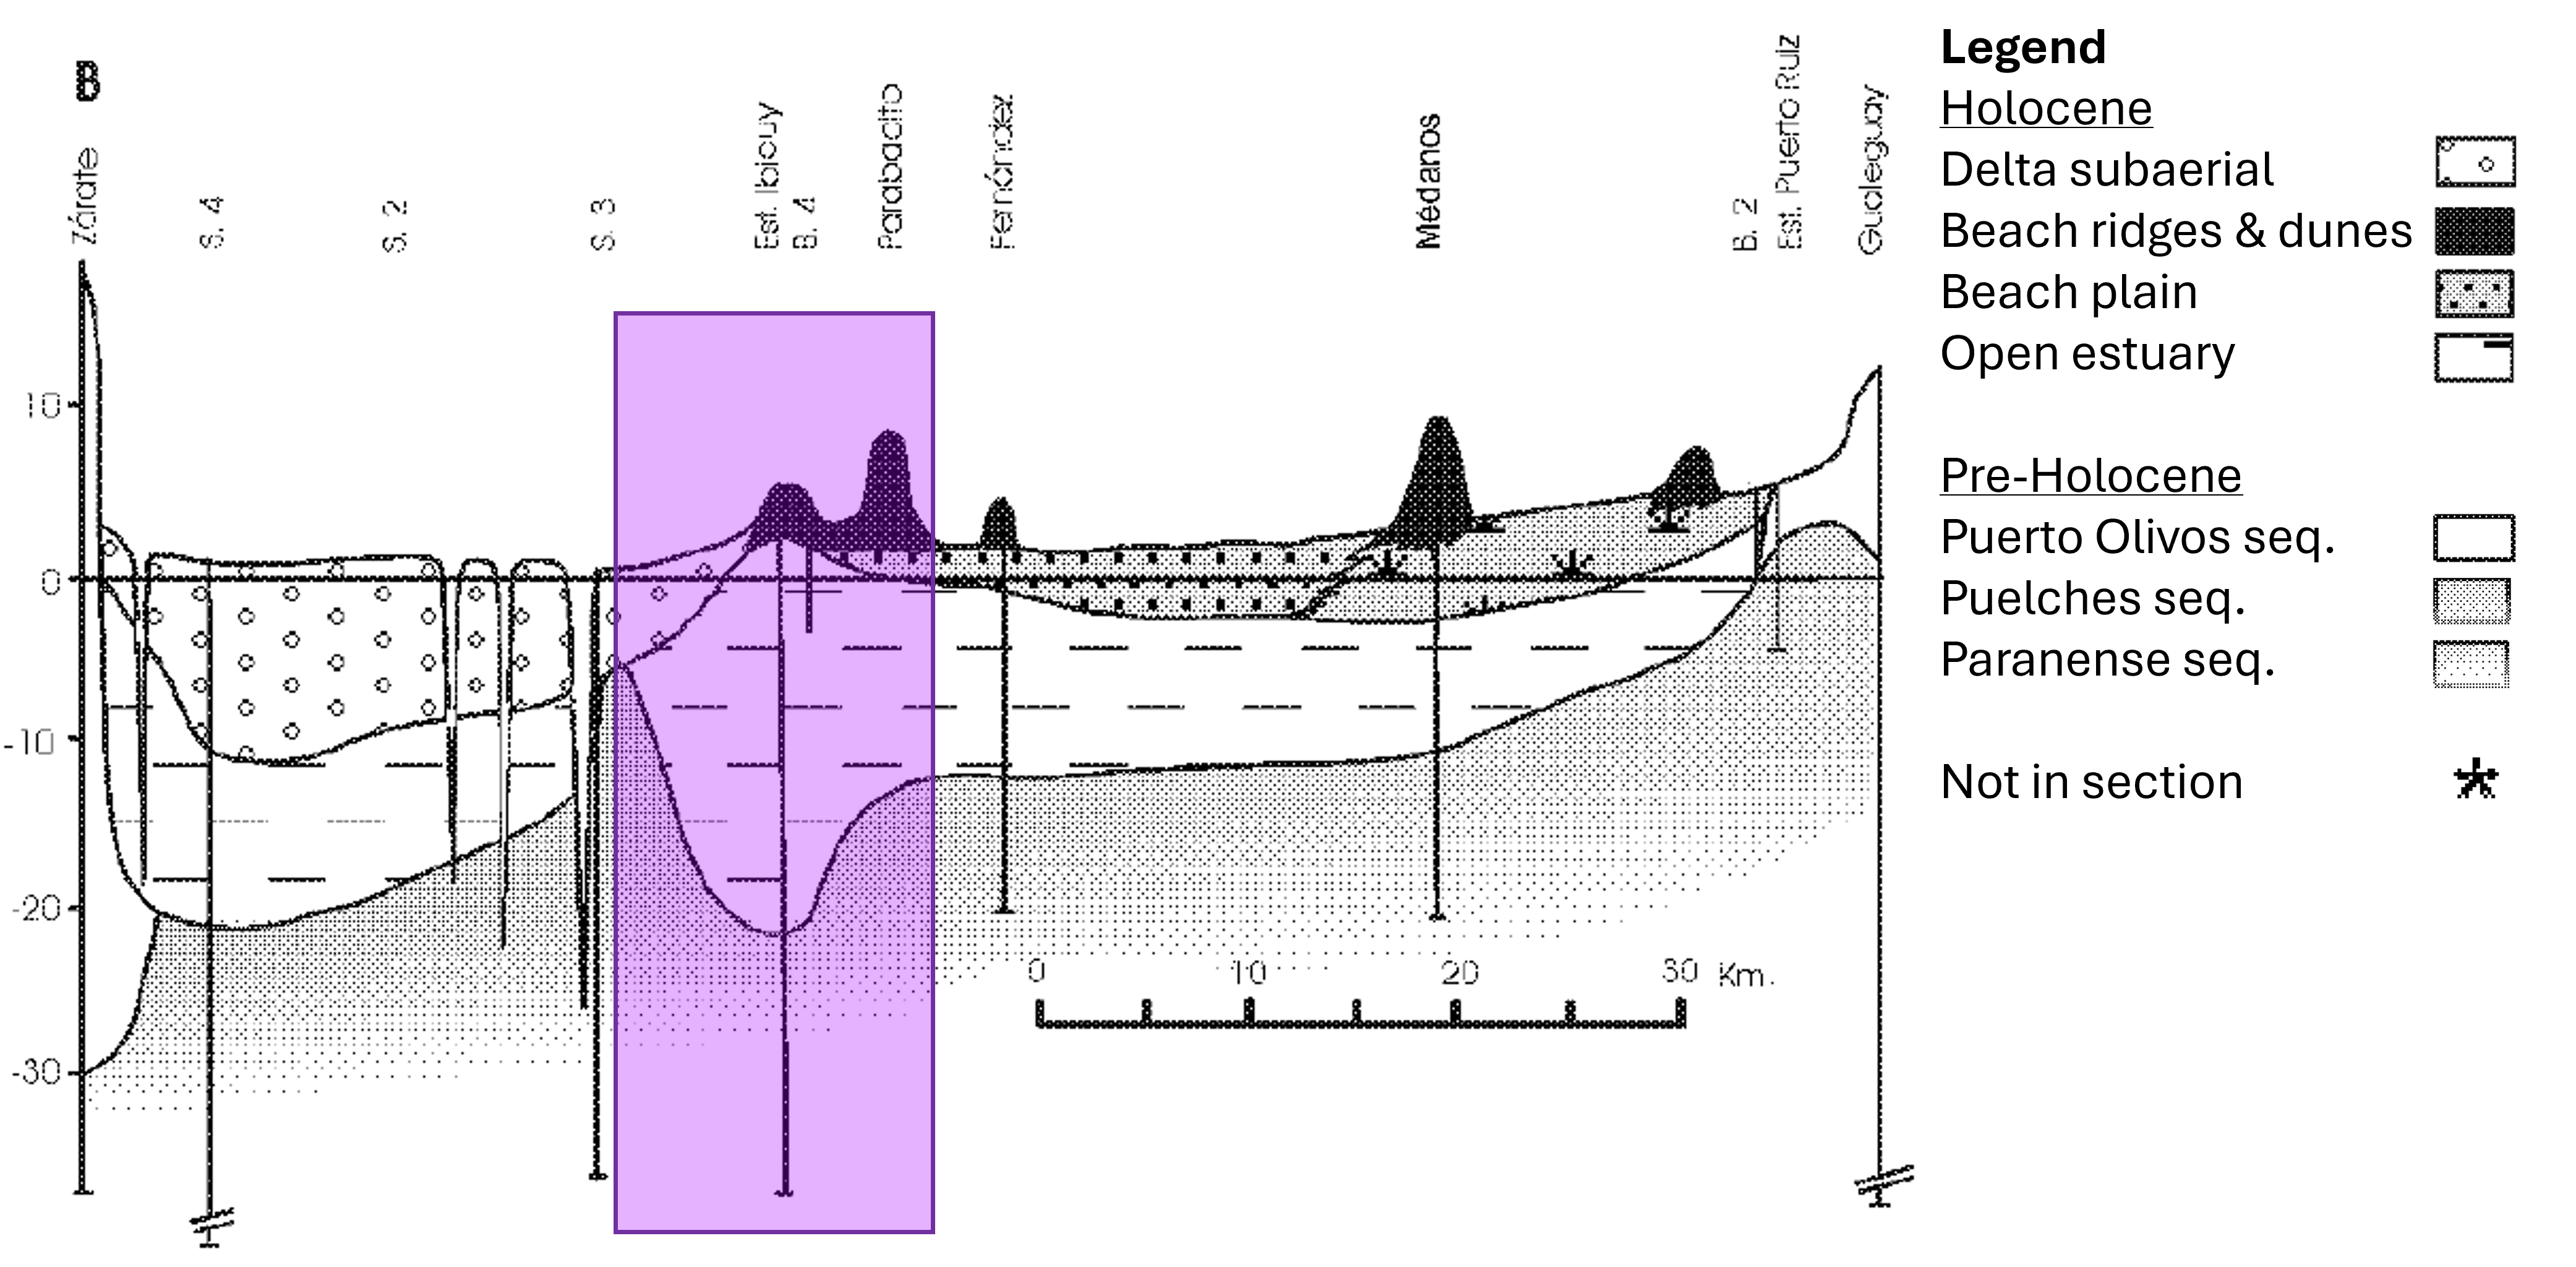
\includegraphics[width=1\linewidth]{figures/ch9/CrossSectionBResults.png}
    \caption{Geological profile of cross section \autocite{joseluiscavallottoEvolucionCambiosAmbientales2005}}
    \label{fig:geolprofile}
\end{figure}

\begin{itemize}
    \item Beach ridges \& dunes: This layer consists of ridge-like beach deposits overlain by dunes. The beach deposists have a maximum thickness of 2 m and are composed mainly of well-sorted fine to medium sands with shell fragments. Light minerals represent 97.8\% of the sand, almost all of which is quartz \autocite{rafaelcordiniContribucionConocimientoGeologia1949}. Radiocarbon dating indicates the deposits formed about 6,400–5,500 years ago, during the mid-Holocene. The ridges represent berm deposits formed by coastal progradation toward the northwest, driven by southeast winds and littoral drift.
    The dunes are up to 11 meters high, especially near Ibicuy, where dune elevations range from 9 to 11 meters and extend 1–2.5 km wide. The dunes consist of well-sorted, fine brown sands composed mostly of quartz (>99\%), with minor feldspars and heavy minerals such as magnetite, zircon, staurolite, and kyanite \autocite{rafaelcordiniContribucionConocimientoGeologia1949}. Thermoluminescence dating shows ages between ~2,800 and <500 years old, indicating several phases of dune formation. Their greatest development on the southeast side shows that, like the underlying beach ridges, they were shaped by southeast winds and continue to be reworked by modern activity \autocite{joseluiscavallottoEvolucionCambiosAmbientales2005}.

    \item Beach plain: The Beach Plain Facies consist of a series of closely spaced beach ridges formed during phases of shoreline retreat and sediment accumulation. The deposits are composed of fine to very fine sands, moderately to well sorted, dominated by quartz (85–90\%) with minor feldspars and few heavy minerals \autocite{rafaelcordiniContribucionConocimientoGeologia1949}. Radiocarbon testing suggests ages between ~2,600 and 1,800 years. The presence of both estuarine shells and freshwater species indicates a transition from estuarine to fluvial conditions as river influence increased \autocite{joseluiscavallottoEvolucionCambiosAmbientales2005}.

    \item Delta subaerial: The subaerial facies of the Paraná Delta developed through the deposition of silty-sandy sediments delivered mainly by the Paraná Guazú and Paraná de las Palmas \autocite{joseluiscavallottoEvolucionCambiosAmbientales2005}. These deposits occur at elevations between 2 m and sea level, with a maximum thickness of 12 m. This is the layer that is drained.
    Mineralogical analyses show a predominance of quartz with minor plagioclase and K-feldspar, plus heavy minerals such as magnetite, hematite, garnet, zircon, tourmaline \autocite{rafaelcordiniContribucionConocimientoGeologia1949}. The age of the unit is debated: radiocarbon dates suggest origin dates between -150 BC and 180 AD, while other authors propose a later origin around 700–750 AD \autocite{joseluiscavallottoEvolucionCambiosAmbientales2005}.
    
    \item Open estuary: The open estuary sediments were deposited during postglacial sea-level rise and were formed at the freshwater–saltwater interface. At the time, seawater flooeded the Río de la Plata river valley \autocite{joseluiscavallottoEvolucionCambiosAmbientales2005}.
    These are olive-green clays to silty clays with thin fine-sand layers, scattered or concentrated shell beds, and fossil content confirming estuarine conditions. The unit is dated to the Holocene, with its base at ~6670 +/- 100 years BC, occurring between –22 and –0 m and reaching up to 20 m thick \autocite{vogelGroningenRadiocarbonDates1969}.
    
    \item Paranense sequence: During the Miocene, large portions of present-day Argentina, Uruguay, Paraguay, southern Brazil, and eastern Bolivia were covered by the Paranense Sea. This was a shallow sea that advanced from the Atlantic into the interior of South America . Its waters left behind marine sediments and fossils and this layer is now known as the Paranense depositional sequence \autocite{tineoReconstructingSouthAmerican2024}.
    
    It is composed mainly of siliciclastic sandstones, mudstones, and bioclastic beds, with thicknesses ranging from a few meters in outcrop to over 100 m. The lower part has mud-dominated offshore deposits with marine fossils, while the upper part is sandier. Studies link the deposits to the Late Miocene (ca. 9.5–6.7 Ma) \autocite{tineoReconstructingSouthAmerican2024}.
\end{itemize}

%Another study focuses on subsurface deposits from Diamante in Entre Ríos to San Fernando in the Buenos Aires province. Based on lithologic, clay mineral, radiocarbon, and outcrop data, the authors propose a depositional model for the region. This geological cross section is shown in figure \ref{fig:depmodel}. The purple area marks the area of interest for this research (Puerto Ibicuy).

%\begin{figure}[H]
%    \centering
   % 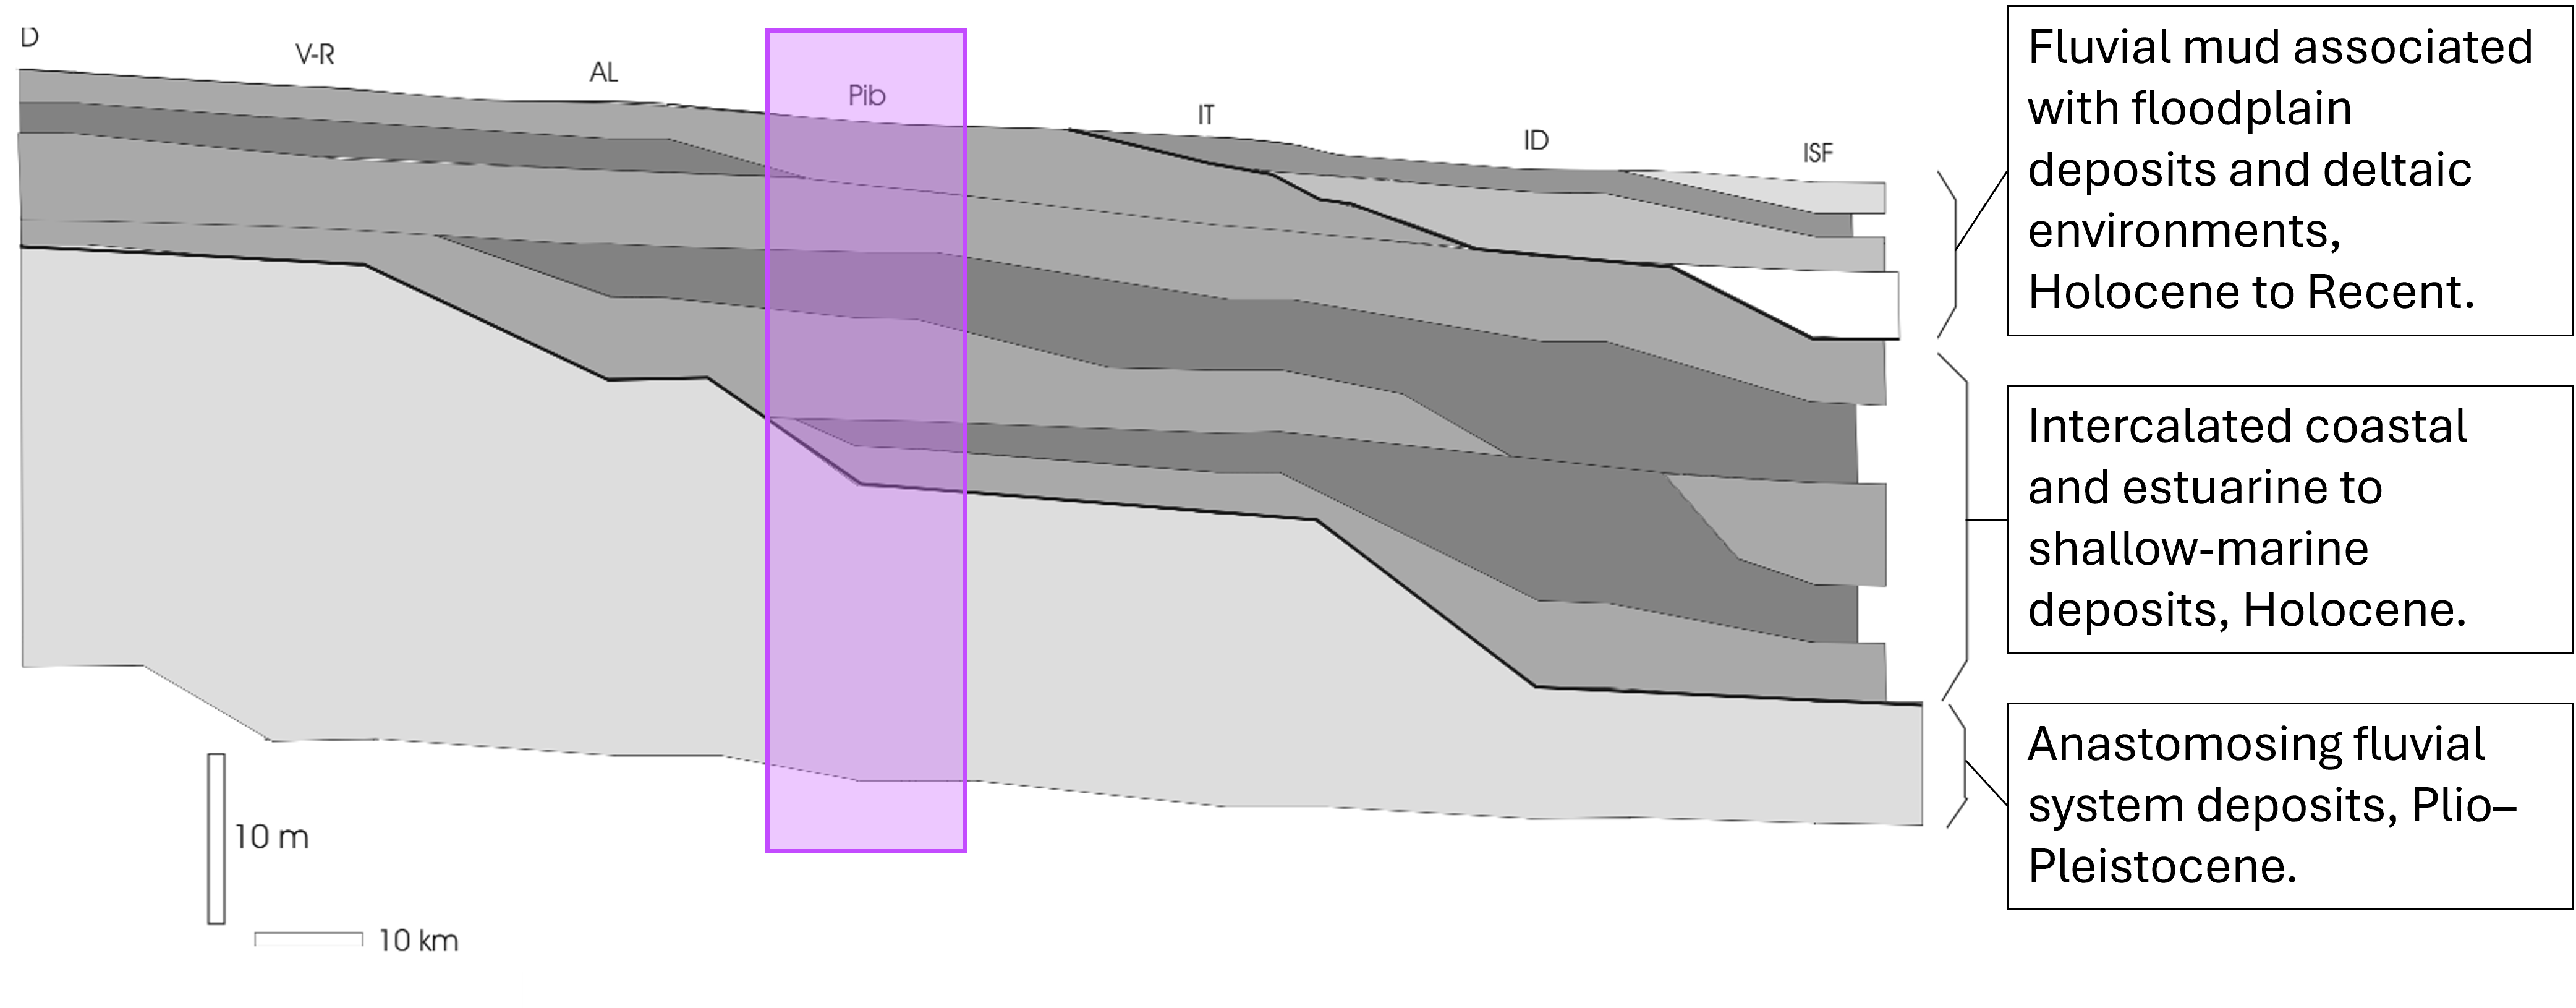
\includegraphics[width=1\linewidth]{figures/ch9/Crosssection2.png}
  %  \caption{Depositional model \autocite{amatoESTRATIGRAFIACUATERNARIASUBSUELO2009}}
  %  \label{fig:depmodel}
%\end{figure}

%As can be seen in the figure, the first layer consists of deltaic and flooplain deposits from the Holocene until recent times. This is in accordance with the geological profile as shown in figure \ref{fig:crosssectiongeo}. Underneath, holocene coastal/estuarine sediments can be found and below there are the Plio–Pleistocene fluvial deposits. The estuarine sediments can also be found in figure \ref{fig:crosssectiongeo}, but a different conclusion was reached for the final layer. \citeauthor{joseluiscavallottoEvolucionCambiosAmbientales2005} conclude that this is a pre-holocene marine deposit from the Miocene Paranense Sea, while here Plio–Pleistocene river deposits are placed below the Holocene sequence.

\subsubsection{Borehole}
In a study conducted by \citeauthor{amatoESTRATIGRAFIACUATERNARIASUBSUELO2009}, a number of boreholes were executed along the lower Paraná \autocite{amatoESTRATIGRAFIACUATERNARIASUBSUELO2009}. One of these boreholes was executed near the area of interest in Puerto Ibicuy. The borehole was interpreted and with this the following soil profile was made.

\begin{figure}[H]
    \centering
    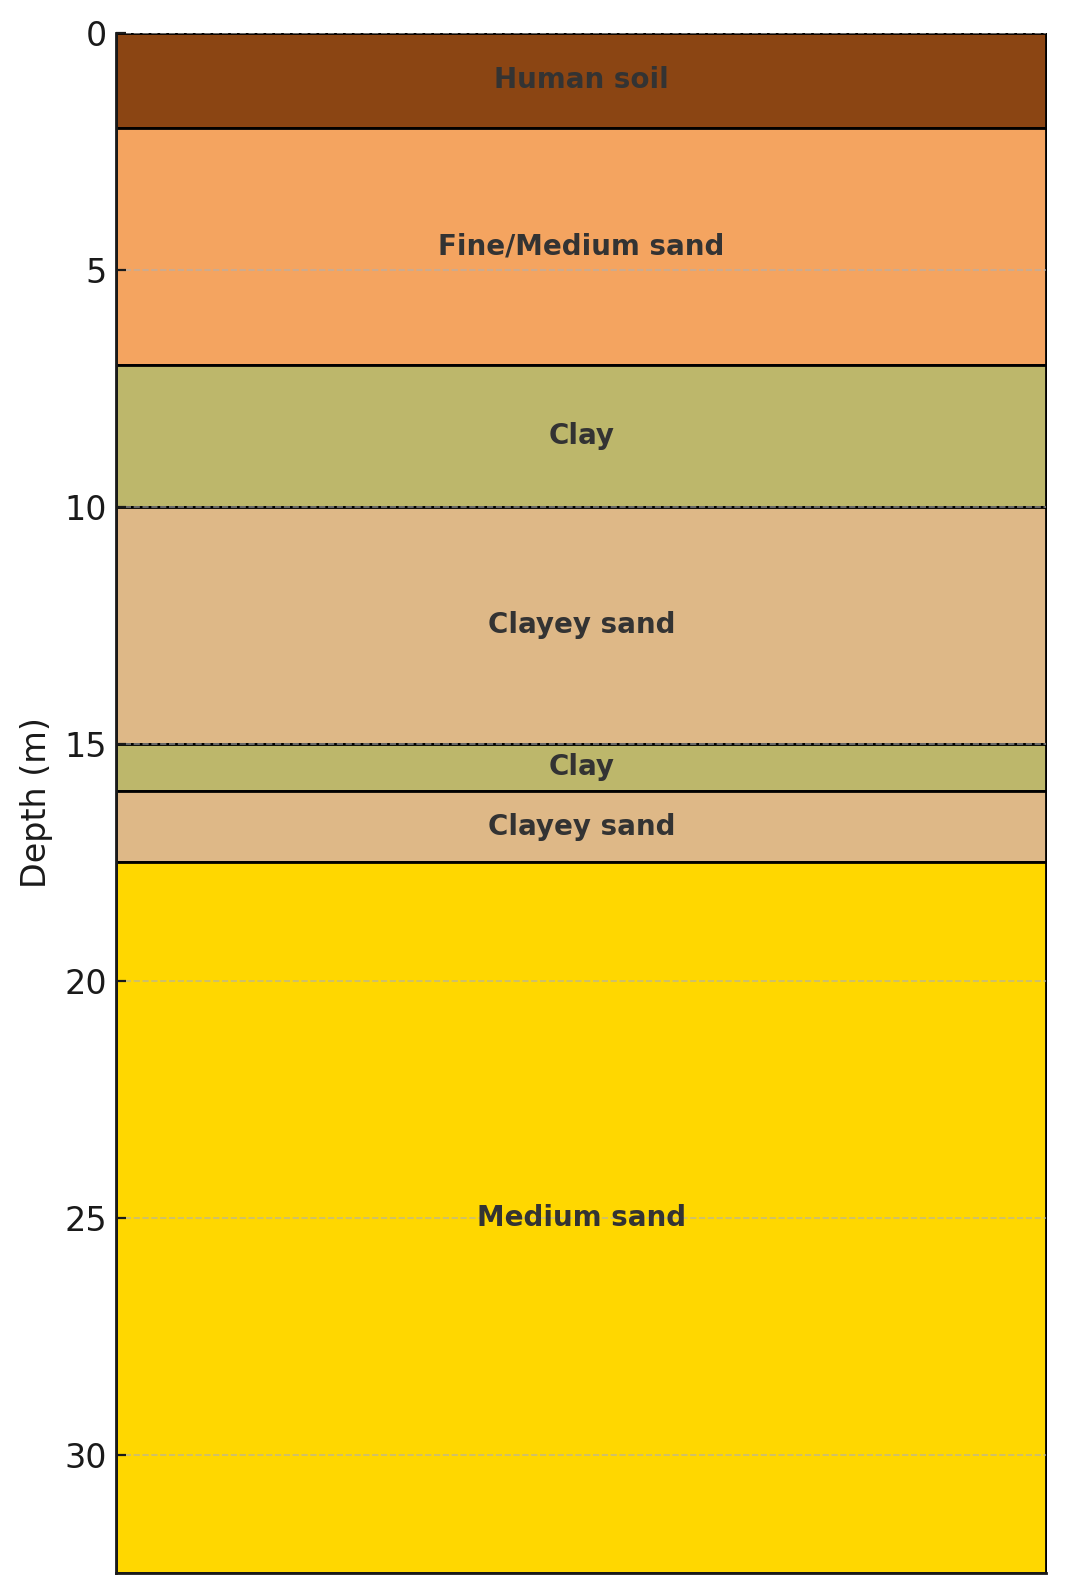
\includegraphics[width=0.45\linewidth]{figures//ch9/Bodemprofiel.png}
    \caption{Borehole profile in Puerto Ibicuy \autocite{amatoESTRATIGRAFIACUATERNARIASUBSUELO2009}}
    \label{fig:borehole}
\end{figure}

\subsection{Characteristics of fracking sand}
\label{sec:Charact. of fs}
Sand used in the fracking process must have fairly specific characteristics in order to be usable for fracking. Silicon sand is mainly used for fracking. This is sand with a grain size between 0.0625 and 2.0 millimeters. The quartz grain content must be higher than 90%. 

Means of transport such as waves and currents in rivers promote the removal of finer or organic particles, thereby ensuring a higher percentage of quartz grains. This is one of the reasons why sand from the Paraná Delta is suitable for fracking.
In addition to erosion by water, the action of wind also influences the characteristics of sand. It causes changes in texture and generally makes quartz sand rounder. 

The specifications for silica sand are written down in the international test standard ISO 13503-2:2006. The important aspects are as follows:

\begin{enumerate}
    \item  Size and distribution of the particles
    \item Shape of the particles
    \item Acid resistance 
    \item Fracture and compressive strength of the grains
    \item Clay and silt content
\end{enumerate}

When it comes to size distributions of the sand particles, the most important is that 90 per cent or more is found in a small size range. Thereby is the size of the particles of less importance and can per badge differ. But when using a sand badge, that badge must have almost exact the same distribution. 

The shape of the sand particles must be round enough and smooth enough to be applicable. Therefore is the system of Krumbrein, W.C. en Sloss, LL. used. This system is shown in Figure \ref{fig:RT}. The norm says that for both roundness as sphericity the value must as least be 0.6. It's important to mention that this procedure is visual and therefore depends on the subjective perception of the person analysing the sample.

\begin{figure}[H]
    \centering
    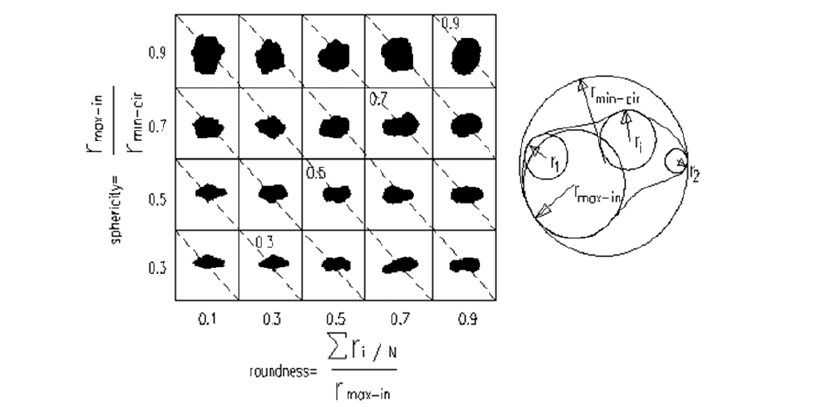
\includegraphics[width=0.75\linewidth]{figures//ch9/roundness.png}
    \caption{Roundness table \autocite{rodriguezParticleShapeQuantities2013}}
    \label{fig:RT}
\end{figure}

Acid solubility testing is used to determine the concentration of soluble elements that contaminate the binder. These elements are typically softer materials that can break down and migrate into the artificially created pore system during fracture closure. This process can lead to conductivity issues within the formation.
To evaluate this are various acids  used of which most are hydrochloric and hydrofluoric acids. These acids dissolve soluble grains such as carbonates, clays, and oxides, while leaving quartz grains intact. Because of this behaviour, industry regulations specify maximum allowable levels of acid-soluble materials that could significantly reduce the permeability of cracks in the wells.
For coarser frac sand with a grain size up to 30/50 mesh, a maximum of 2\% acid-soluble content is permitted. For finer sands, this limit increases to 3\%, as shown in \ref{tab:acid} below.

\begin{table}[h!]
\centering
\begin{tabular}{|c|c|c|}
\hline
\textbf{Particle size (ASTM)} & \textbf{Particle size (mm)} & \textbf{Max. solubility (\% by weight)} \\ \hline
6/12 to 30/50 & 1.68/3.36 to 0.30/0.60 & 2.0 \\ \hline
40/70 to 70/140 & 0.21/0.42 to 0.10/0.21 & 3.0 \\ \hline
\end{tabular}
\caption{Recommended maximum acid solubility \autocite{secretariadepoliticamineraArenasParaFracking2019}}
\label{tab:acid}
\end{table}

For the compressive strength of grains is a test conducted which puts a pressure on the sand particles and then sieves the sample to look which percentage of the particles go trough a certain sieve. This percentage of breaking particles in combination with the known applied pressure tells us which pressure the sand can withstand when using it for making cracks.
The permeability of the fracks in the oil sources drops rapidly if the percentages of cracking sand particles and clay/silt particles is too high. 

\subsubsection{Characteristics of Ibicuy specific}

The sand of the Ibicuy region in the province of the Entre Rios is mostly composed of quarts (86\%). But the sand is quite polluted by iron minerals. The percentage of heavy minerals is very low (0.3\%). This is one of the reasons that the sand is washed before transporting it to the fracking plants \autocite{secretariadepoliticamineraArenasParaFracking2019}. 

\subsection{Consequences of dry sand mining}
The effects of dry sand mining can be diverse. This section combines various reports on dry sand mining as well as knowledge that arises from stakeholder interviews to provide an overview of the consequences that can be linked to this activity.

\subsubsection{Effects on natural habitats}
The most obvious effects due to dry sand mining have to do with the natural environment. As became clear in stakeholder interviews, sand mining leads to the removal of several meters of top soil. This operation requires clearing land of their natural cover: forests or grasslands are removed.

During the interview, the YPF sand mine manager showed two sites where sand mining activities were stopped due to exhaustion of the sand resource. He explained that after mining activities are completed, the areas are left uninterrupted and are thus `given back to nature'. Figure \ref{fig:aftermining} shows the current condition of two former sand mining locations. On the left, activities ceased one year ago and on the right, mining has stopped since four years. The mined areas can be seen in the back of the photos, the sand in the foreground is not part of these sites.

\begin{figure}[H]
    \centering
    \includegraphics[width=1\linewidth]{figures/ch9/Aftermining.png}
    \caption{The state of `finished' locations: after 1 year (left) and after 4 years (right) (Own work)}
    \label{fig:aftermining}
\end{figure}

From figure \ref{fig:aftermining}, it seems that the natural cover (grasslands and forests) has recovered quite quickly in this case. It must however be noted that changes to the original natural environment can still be severe: the original soil profile has drastically changed, meaning that even though a new natural cover has emerged, original species might not be able to survive anymore.

Examples of this can be found in the United States of America: over the past decades, the Dunes Sagebrush Lizard has seen more than 95\% of its original habitat in Texas and New Mexico disappear. This is due to the oil industry and the large scale sand mining operations that support it. In 2024, the species was listed as endangered by the U.S. Fish and Wildlife Service \autocite{centerforbiologicaldiversityLegalInterventionLaunched2025}. Sand mining leads to permanent removal of habitats, which means that letting natural cover grow back may not be enough for species like these to return.

\subsubsection{Social effects}
The most frequently voiced concerns of stakeholders is the poor conditions of roads, especially the provincial RP45 that forms the entrance to the town, caused by intense heavy truck traffic. These comments were confirmed during the field trip, since many potholes were observed along the entire route.

The poor road conditions are not only uncomfortable but also dangerous. In fact, in 2020 alone, ten people lost their lives on the roads that form part of the sand transport routes. The situation has lead to protesting citizens and to blockages of the national highway 12 \autocite{novasImpactoAmbientalOculto2022}.

Other possible negative effects on people living near the sand mines include noise pollution and light pollution, although these concerns were not raised by stakeholders that were interviewed.

\subsubsection{Economic effects}
In the short term, sand mining can contribute to the economic development of an area. Jobs are created and the government can profit through direct and indirect taxation of the activities. However, since all sand mining activities face a natural end (the YPF mine operator indicated that his mine had resources to stay open for 8 more years), positive economic effects do not persists in the long term. A closer look at the situation in Ibicuy reveals more economic troubles related to sand mining.

The Argentinian mining codes dictate that so-called `third-category mines', such as silica sand mines, belong solely to the owner. The government therefore does not receive royalties for exploitation of the areas but instead charges taxes based on volumes \autocite{novasImpactoAmbientalOculto2022}. Instead, the mayor and YPF mine manager indicated that both provincial and municipal taxes are in place. The transport is taxed and each truck pays a tax based on the mass it carries.

From 2019 until 2023, the provincial government of Entre Ríos chose to not adjust the mining taxes, such that the provincial income from these taxes was approximately stable at 400 million pesos per year. However, this period was marked by high inflation and strong devaluation of the Argentine peso \autocite{bellatoEntreRiosFrigerio2025}. In December 2019, at the start of the previous administration's term, 400 million pesos equaled approximately 3 million Euros. At the end of their ruling, in December 2023, the same sum was worth 440.000 Euros, enough for repaving around 1 kilometer of road that is in `fair' condition, by U.S. standards \autocite{crumbCostRoadMaintenance2024}. 

The new provincial government tried to strike a deal with fossil fuel companies to secure investments in infrastructure. After this turned out fruitless, taxes were raised by a factor six in May 2025. As of today, trucks pay 2250 Argentine pesos per ton, a rate that, according to the president of Entre Ríos’ tax authority, still falls short of covering the province’s road repair costs \autocite{crumbCostRoadMaintenance2024}. 

Both the province and municipality charge taxes on transported sand. However, in 2022, municipal mining taxes were only around one tenth of the taxes the province charged on the activity \autocite{novasImpactoAmbientalOculto2022}. At 37 million pesos, the municipal taxes are too low to contribute significantly to road reparations.

\subsubsection{Air quality and health}
During mining, washing and transport processes, silica-rich sands release airborne crystalline silica particles (silica dust). When the silica dust is inhaled, it can contribute to respiratory diseases like silicosis and lung cancer \autocite{physiciansforsocialresponsibilityCompendiumScientificMedical2023}. In 2013, the National Institute for Occupational Safety and Health (NIOSH) tested silica concentrations in 11 sand mining locations in the US. They found that 79\% of samples exceeded the recommended limit, and in some cases the found concentrations even exceeded limits that hold while wearing protection masks \autocite{fogliaSedArena2023}. Effects of silica dusts on nearby communities are a topic of discussion. A 2017 study researched crystalline silica concentrations in homes within 800 m of sand mining activities and concluded that exposure seems unlikely to cause chronic health problems to these communities, because of relatively low concentrations \autocite{}. However, in January 2021, a ban on frack sand mining in Winona County, Minnesota, US, was upheld by the Supreme Court. The ban was put in place by the county out of concerns about environmental and health impacts \autocite{physiciansforsocialresponsibilityCompendiumScientificMedical2023}.

\subsubsection{Washing operations}
After the sand is mined, it is washed to clean it from unwanted substances such as clay and organic material. For this, large amounts of groundwater are used. In Ibicuy, the sand miners use water from the Talavera formation, which is the same water that flows out of the tap. 

Sand mining companies are reluctant to share information about extracted groundwater volumes. However, in 2020, an environmental information lawsuit revealed 33 documents with specifics. At the time there were 5 sand-washing installations near Ibicuy that together extracted 400 million liters of groundwater per month from the Talavera formation. In comparison, the drinking water cooperation extracts 30 million liters per month in winter and 60 million liters per month in the summer \autocite{fogliaSedArena2023}. Considering the further increase in mining activities since 2020, it seems likely that even more groundwater is extracted now. 

In addition to drinking water competition, the sand washing installations have the capacity to pollute water reservoirs, an effect that is already noticeable in Ibicuy. In june 2022, the local water treatment company reported manganese concentrations of 0.75 mg per liter, whereas the recommended water concentration limit for lifetime exposure is 0.3 mg/L. Further, iron concentrations of 0.93 mg and 1.10 mg were found, an increase of 2200\% as compared to the historic value of 0.05 mg. Additionally, flocculants such as polyacrylamide are used to clump together clay particles and other fine suspended solids. Polyacrylamide can infiltrate into the surface and the underground and can break down into acrylamide during drying \autocite{fogliaSedArena2023}. The WHO warns that this substance is genotoxic, capable of damaging genetic material, and carcinogenic and that acrylamide is therefore a human health concern

\subsection{Recommendations and mitigation strategies}
Meer overheidsingrijpen nodig? Zie interview burgemeester: The judiciary forced the government to get involved: do controls, plan and regulate. Now there’s
a limit to extract, approx. 2 – 3 m. Before, there wasn’t.
En sed de arena report, overheid niet proactief genoeg

%https://www.unep.org/resources/report/sand-and-sustainability-10-strategic-recommendations-avert-crisis
%https://aapepyg.com/2022/11/23/fracking_entre_rios/#_edn4


While significant strides are taken to implement
nature-based solutions (NbS) against climate change
challenges, it is important to note that NbS requires large
volume of sand. Additionally, NbS may take time to have
the desired effect. Thus in some cases, grey structures
(i.e., concrete) may be necessary in the mean time to
address challenges in the short- to medium-term. In the
context of extreme heat and its impacts on cities, NbS
will also be instrumental to promote building designs and
materials that require neither concrete infrastructure nor
sand (UNEP 2021b). Climate change induced pressures,
such as temperature stress and precipitation, will also
speed up the degradation of existing infrastructure and
the need for upgrading or replacement
https://www.unep.org/resources/report/sand-and-sustainability-10-strategic-recommendations-avert-crisis

Op basis van uitgebreid, door deskundigen beoordeeld bewijsmateriaal concludeerde het Compendium van wetenschappelijke, medische en media-bevindingen die de risico's en schade van fracking aantonen, dat het niet mogelijk is om de techniek van de winning van onconventionele koolwaterstoffen 17Sed de Arena 2023 I Valeria Foglia en de daarmee samenhangende winningsactiviteiten niet mogelijk is zonder dat dit een bedreiging vormt voor de menselijke gezondheid, de lucht, het water, de economische vitaliteit op lange termijn, de biodiversiteit en de seismische en klimatologische stabiliteit. SED DE ARENA


Naar aanleiding van herhaalde klachten van inwoners heeft de Federale Rechtbank van Gualeguaychú in mei van dit jaar de sluiting van negen kwartszandgroeven in Ibicuy en Gualeguaychú voor 45 dagen bevolen vanwege herhaalde milieuovertredingen. Onlangs werd ook de definitieve sluiting bevolen van Cristamine SA , een van de belangrijkste bedrijven van het land, vanwege milieuvervuiling. Deze maatregel onderstreept de noodzaak om de sociale en milieueffecten van fracking in Argentinië uitgebreid te onderzoeken . WEBSITE